\section{Modules, homomorphisms and exact sequences}
\begin{ex}
    If $A$ is an abelian group and $n>0$ an integer such that $na=0$ for all $a\in A$, then $A$ is a unitary $Z_{n}$-module, with the action of $Z_{n}$ on $A$ given by $\bar{k}a=ka$, where $k\in \mathbf{Z}$ and $k\mapsto \bar{k}\in Z_{n}$ under the canonical projection $\mathbf{Z}\to Z_{n}$.
\end{ex}

$$ $$

\begin{ex}
    Let $f:A\to B$ be an $R$-module homomorphism.
    \begin{enumerate}[(a)]
        \item $f$ is a monomorphism if and only if for every pair of $R$-module homomorphisms $g,h:D\to A$ such that $fg=fh$, we have $g=h$.
        \item $f$ is an epimorphism if and only if for every pair of $R$-module homomorphisms $k,t:B\to A$ such that $kf=tf$, we have $k=t$.
    \end{enumerate}
\end{ex}

$$ $$

\begin{ex}
    Let $I$ be a left ideal of a ring $R$ and $A$ an $R$-module.
    \begin{enumerate}[(a)]
        \item If $S$ is a nonempty subset of $A$, then $IS=\{\sum\limits_{i=1}^{n}r_{i}a_{i}|n\in \mathbf{N}^{*}; r_{i}\in I;a_{i}\in S\}$ is a submodule of $A$. Note that if $S=\{a\}$, then $IS=Ia=\{ra|r\in I\}$.
        \item If $I$ is a two-sided ideal, then $A /IA$ is an $R /I$-module with the action of $R /I$ given by $(r+I)(a+IA)=ra+IA$.
    \end{enumerate}
\end{ex}

$$ $$

\begin{ex}
    If $R$ has identity, then every unitary cyclic $R$-module is isomorphic to an $R$-module of the form $R /J$, where $J$ is a left ideal of $R$.
\end{ex}

$$ $$

\begin{ex}
    If $R$ has identity, then a nonzero unitary $R$-module $A$ is \textbf{simple} if its only submodules are 0 and $A$.
    \begin{enumerate}[(a)]
        \item Every simple $R$-module is cyclic.
        \item If $A$ is simple every $R$-module endomorphism is either the zero map of and isomorphism.
    \end{enumerate}
\end{ex}

$$ $$

\begin{ex}
    A finitely generated $R$-module need not to be finitely generated as an an abelian group.
\end{ex}

$$ $$

\begin{ex}
    \begin{enumerate}[(a)]
        \item If $A$ and $B$ are $R$-modules, then the set $\mathrm{Hom}_{R}(A,B)$ of all $R$-module homomorphisms $A\to B$ is an abelian group with $f+g$ given on $a\in A$ by $(f+g)(a)=f(a)+g(a)\in B$. The identity element is the zero map.
        \item $\mathrm{Hom}_{R}(A,B)$ is a ring with identity, where multiplication is composition of functions. $\mathrm{Hom}_{R}(A,B)$ is called the \textbf{endomorphism ring} of $A$.
        \item $A$ is a left $\mathrm{Hom}_{R}(A,A)$-module with $fa$ defined to be \[f(a)(a\in A), f\in \mathrm{Hom}_{R}(A,A)\]
    \end{enumerate}
\end{ex}

$$ $$

\begin{ex}
    Prove that the obvious analogues of Theorem I.8.10 and Corollary I.8.11 are valid for $R$-modules.
\end{ex}

$$ $$

\begin{ex}
    If $f:A\to A$ is an $R$-module homomorphism such that $ff=f$, then \[A=\mathrm{Ker}f\oplus\mathrm{Im}f\]
\end{ex}

$$ $$

\begin{ex}
    Let $A,A_{1},\dots, A_{n}$ be $R$-modules. Then $A\cong A_{1}\oplus\cdots\oplus A_{n}$ if and only if for each $i=1,2,\dots,n$ there is an $R$-module homomorphism $\varphi_{i}:A\to A$ such that $\mathrm{Im}\varphi_{i}\cong A_{i}$; $\varphi_{i}\varphi_{j}$ for $i\neq j$; and $\varphi_{1}+\varphi_{2}+\cdots+\varphi_{n}=1_{A}$.
\end{ex}

$$ $$

\begin{ex}
    \begin{enumerate}[(a)]
        \item If $A$ is a module over a commutative ring $R$ and $a\in A$, then $\mathcal{O}_{a}=\{r\in R|ra=0\}$ is an ideal of $R$. If $\mathcal{O}_{a}\neq 0$, $a$ is said to be a \textbf{torsion element} of $A$.
        \item if $R$ is an integral domain, then the set $T(A)$ of all torsion elements of $A$.($T(A)$ is called the \textbf{torsion submodule}.)
        \item Show that (b) may be false for a commutative ring $R$, which is not an integral domain.
        
        In (d) - (f) $R$ is an integral domain.
        \item If $f:A\to B$ is an $R$-module homomorphism, then $f(T(A))\subset T(B)$; hence the restriction $f_{T}$ of $f$ to $T(A)$ is an $R$-module homomorphism $T(A)\to T(B)$.
        \item If $0\to A\xrightarrow{f} B\xrightarrow{g} C$ is an exact sequence of $R$-module, then so is $0\to T(A)\xrightarrow{fT} T(B)\xrightarrow{gT}T(C)$.
        \item If $g:B\to C$ is an $R$-module epimorphism, then $g_{T}:T(B)\to T(C)$ need not be an epimorphism.
    \end{enumerate}
\end{ex}

$$ $$

\begin{ex}
    (The Five Lemma). Let
    \begin{figure}[H]\centering
        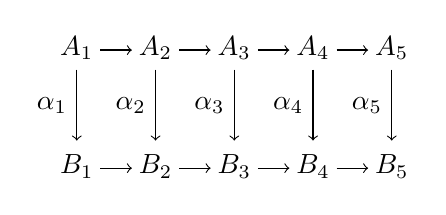
\begin{tikzpicture}
            \node [above] at (0,0) {$B_{1}$};
            \node [above] at (1,0) {$B_{2}$};
            \node [above] at (2,0) {$B_{3}$};
            \node [above] at (3,0) {$B_{4}$};
            \node [above] at (4,0) {$B_{5}$};
            \node [above] at (0,1.5) {$A_{1}$};
            \node [above] at (1,1.5) {$A_{2}$};
            \node [above] at (2,1.5) {$A_{3}$};
            \node [above] at (3,1.5) {$A_{4}$};
            \node [above] at (4,1.5) {$A_{5}$};
            \draw [->] (0.3,0.25) to (0.7,0.25);
            \draw [->] (1.3,0.25) to (1.7,0.25);
            \draw [->] (2.3,0.25) to (2.7,0.25);
            \draw [->] (3.3,0.25) to (3.7,0.25);
            \draw [->] (0.3,1.75) to (0.7,1.75);
            \draw [->] (1.3,1.75) to (1.7,1.75);
            \draw [->] (2.3,1.75) to (2.7,1.75);
            \draw [->] (3.3,1.75) to (3.7,1.75);
            \draw [->] (0,1.5)-- node [left, pos=0.5]{$\alpha_{1}$} (0,0.6);
            \draw [->] (1,1.5)-- node [left, pos=0.5]{$\alpha_{2}$} (1,0.6);
            \draw [->] (2,1.5)-- node [left, pos=0.5]{$\alpha_{3}$} (2,0.6);
            \draw [->] (3,1.5)-- node [left, pos=0.5]{$\alpha_{4}$} (3,0.6);
            \draw [->] (4,1.5)-- node [left, pos=0.5]{$\alpha_{5}$} (4,0.6);
        \end{tikzpicture}
    \end{figure}
    be a commutative diagram of $R$-module homomorphisms, with exact rows. Prove that:
    \begin{enumerate}[(a)]
        \item $\alpha_{1}$ an epimorphism and $\alpha_{2},\alpha_{4}$ monomorphisms $\Rightarrow$ $\alpha_{3}$ is a monomorphism;
        \item $\alpha_{5}$ a monomorphism and $\alpha_{2},\alpha_{4}$ epimorphisms $\Rightarrow$ $\alpha_{3}$ is an epimorphism.
    \end{enumerate}
\end{ex}

$$ $$

\begin{ex}
    \begin{enumerate}[(a)]
        \item If $0\to A\to B\xrightarrow{f} C\to 0$ and $0\to C\xrightarrow{g} D\to D\to E\to 0$ are short exact sequences of modules, then the sequence $0\to A\to B\xrightarrow{gf}D \to E\to 0$ is exact.
        \item Show that every exact sequence may be obtained by splicing together suitable short exact sequences as in (a).
    \end{enumerate}
\end{ex}

$$ $$

\begin{ex}
    Show that isomorphism of short exact sequences in an equivalence relation.
\end{ex}

$$ $$

\begin{ex}
    If $f:A\to B$ and $g:B\to A$ are $R$-module homomorphisms such that $gf=1_{A}$, then $B=\mathrm{Im}f\oplus \mathrm{Ker}g$.
\end{ex}

$$ $$

\begin{ex}
    Let $R$ be a ring and $R^{op}$ its opposite ring. If $A$ is a left $R$-module, then $A$ is a right $R^{op}$-module such that $ra=ar$ for all $a\in A, 4\in R, r\in R^{op}$.
\end{ex}

$$ $$

\begin{ex}
    \begin{enumerate}[(a)]
        \item If $R$ has an identity and $A$ is an $R$-module, then there are submodules $B$ and $C$ of $A$ such that $B$ is unitary, $RC=0$ and $A=B\oplus C$.
        \item Let $A_{1}$ be another $R$-module, with $A_{1}=B_{1}\oplus C_{1}$ ($B_{1}$ unitary, $RC=0$), If $f:A\to A_{1}$ is an $R$-module homomorphism then $f(B)\subset B_{1}$ and $f(C)\subset C_{1}$.
        \item If the map $f$ of part (b) is an epimorphism, then so are $f|B:B\to B_{1}$ and $f|C:C\to C_{1}$.
    \end{enumerate}
\end{ex}

$$ $$

\begin{ex}
    Let $R$ be a ring without identity. Embed $R$ in a ring $S$ with identity and charateristic zero as in the proof of Theorem III.1.10. Identify $R$ with its image in $S$.
    \begin{enumerate}[(a)]
        \item Show that every element of $S$ may be uniquely expressed in the form $r1_{S}+n1_{S}(r\in R, n\in \mathbf{Z})$.
        \item If $A$ is an $R$-module and $a\in A$, show that there is a unique $R$-module homomorphism $f:S\to A$ such that $f(1_{S})=a$.
    \end{enumerate}
\end{ex}